\documentclass[11pt]{article}
\usepackage[pdftex]{graphicx}

\begin{document}
\title{Sieci neuronowe. Projekt}
\author{Micha� Dettlaff}
\maketitle


\section{Wprowadzenie}

\noindent
Celem rozpatrywanego problemu s� w�a�nie...

$f(x) = \frac{1}{4000} \sum_{i=1}^n {x_i}^{2} - \prod_{i=1}^n cos(x_i / \sqrt{i}) +1$


\section{Metodologia}
\noindent
Metodologia...


\section{Wyniki}

Proste regu�y rozmyte
\begin{center}
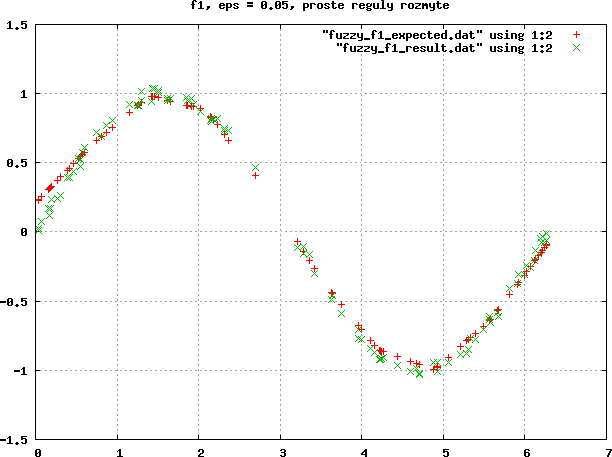
\includegraphics[scale=0.5]{fuzzy_f1}\newline
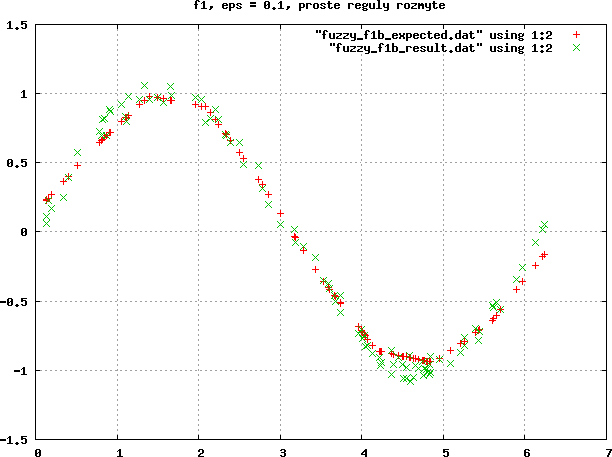
\includegraphics[scale=0.5]{fuzzy_f1b}\newline
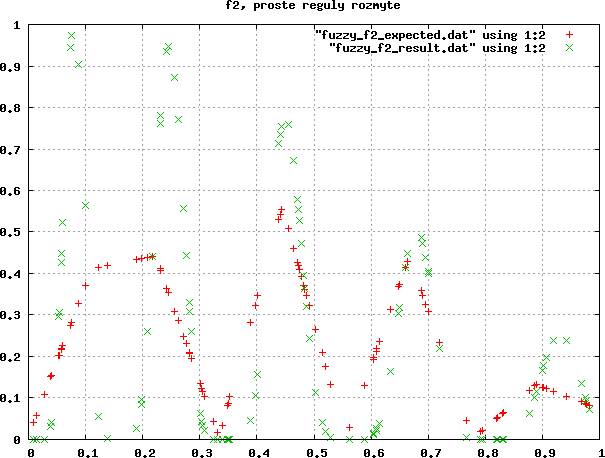
\includegraphics[scale=0.5]{fuzzy_f2}\newline
\end{center}

\newpage
Algorytm propagacji wstecznej
\begin{center}
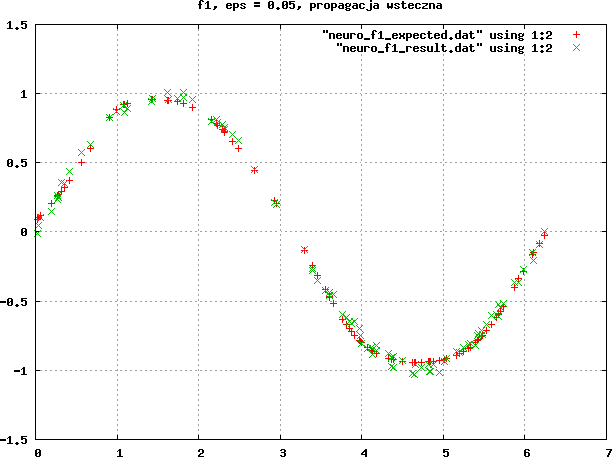
\includegraphics[scale=0.5]{neuro_f1}\newline
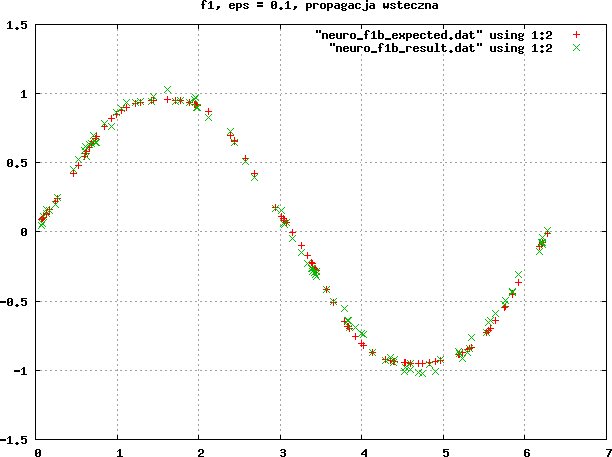
\includegraphics[scale=0.5]{neuro_f1b}\newline
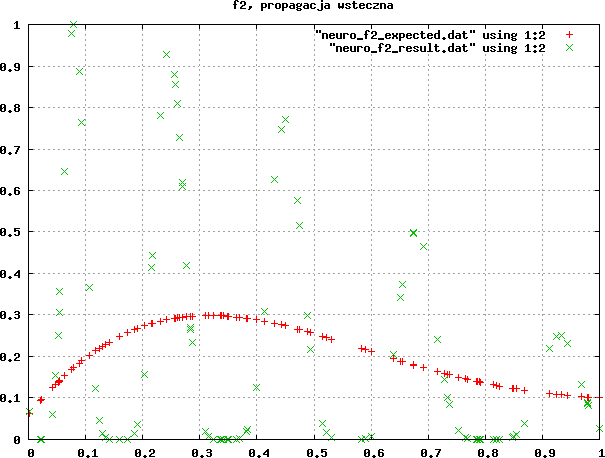
\includegraphics[scale=0.5]{neuro_f2}\newline
\end{center}


\end{document}
